\documentclass[12pt]{article}
\usepackage{amsmath}
\usepackage{amssymb}
\usepackage[letterpaper,top=0.85in,bottom=1in,left=0.75in,right=0.75in,centering]{geometry}
%\usepackage{fancyhdr}
\usepackage{enumerate}
%\usepackage{lastpage}
\usepackage{multicol}
\usepackage{graphicx}

\reversemarginpar

%\pagestyle{fancy}
%\cfoot{}
%\lhead{Math 1560}\chead{Test \# 1}\rhead{May 18th, 2017}
%\rfoot{Total: 10 points}
%\chead{{\bf Name:}}
\newcommand{\points}[1]{\marginpar{\hspace{24pt}[#1]}}
\newcommand{\skipline}{\vspace{12pt}}
%\renewcommand{\headrulewidth}{0in}
\headheight 30pt

\newcommand{\di}{\displaystyle}
\newcommand{\abs}[1]{\lvert #1\rvert}
\newcommand{\len}[1]{\lVert #1\rVert}
\renewcommand{\i}{\mathbf{i}}
\renewcommand{\j}{\mathbf{j}}
\renewcommand{\k}{\mathbf{k}}
\newcommand{\R}{\mathbb{R}}
\newcommand{\aaa}{\mathbf{a}}
\newcommand{\bbb}{\mathbf{b}}
\newcommand{\ccc}{\mathbf{c}}
\newcommand{\dotp}{\boldsymbol{\cdot}}
\newcommand{\bbm}{\begin{bmatrix}}
\newcommand{\ebm}{\end{bmatrix}}                   
\DeclareMathOperator{\sech}{sech}                  
\begin{document}


\author{Instructor: Sean Fitzpatrick}
\thispagestyle{empty}
\vglue1cm
\begin{center}
{\bf MATH 2565 - Tutorial \#4 Solutions}
\end{center}


\textbf{Additional practice problems:}
\begin{enumerate}
\item Evaluate the improper integral, if possible:

\begin{enumerate}
 \item $\di \int_0^\infty x^2e^{-2x}\,dx$
 
 Using integration by parts,
 \begin{align*}
  \int x^2e^{-2x}\,dx &= -\frac12 x^2e^{-2x}+\int xe^{-2x}\,dx\\
  & = -\frac12 x^2e^{-2x} -\frac12 xe^{-2x}+\int e^{-2x}\,dx\\
  & = -\frac12 x^2e^{-2x}-\frac12 xe^{-2x}-\frac12 e^{-2x}+C.
 \end{align*}
The improper integral is thus
\begin{align*}
\int_0^\infty x^2e^{-2x}\,dx &= \lim_{b\to\infty}\int_0^b x^2e^{-2x}\,dx\\
& = \lim_{b\to\infty}\left(\left.-\frac12 e^{-2x}(x^2+x+1)\right|_0^b\right)\\
& = \lim_{b\to \infty}\left(-\frac12 e^{-2b}(b^2+b+1)+\frac12 e^0(0^2+0+1)\right)\\
& = \frac12.
\end{align*}
(Note that $\lim_{b\to\infty}b^ke^{-2b}=0$ for any positive integer $k$, using l'Hospital's rule.)

 \item $\di \int_0^1 \frac{\sqrt{x}+1}{x}\,dx$
 
 Since $\dfrac{\sqrt{x}+1}{x}=\dfrac{1}{\sqrt{x}}+\dfrac{1}{x}$ and $\di\int_0^1 \frac1x \,dx$ diverges, the integral diverges.
 \end{enumerate}  

 \item Determine if the improper integral converges or diverges:

 \begin{enumerate}
  \item $\di \int_0^\infty \frac{1}{\sqrt{x^3+2x^2+5}}\,dx$
  
  Note that for $x\geq 0$, $x^3+2x^2+5\geq 5>0$, so we do not need to worry about the integral being improper due to a vertical asymptote. Thus, we look at the behaviour as $x\to \infty$. For $x$ large, we have
  \[
  \frac{1}{\sqrt{x^3+2x^2+5}} \approx \frac{1}{\sqrt{x^3}}=\frac{1}{x^{3/2}}.
  \]
  Since $\int_1^\infty \frac{1}{x^{3/2}}\,dx$ converges, we suspect that our original integral does as well. Since $2x^2+5>0$ for all $x$, we see that $\dfrac{1}{\sqrt{x^3+2x^2+5}} <\frac{1}{x^{3/2}}$, so the integral converges by direct comparison with $g(x)=x^{-3/2}$.
  
  \item $\di \int_1^\infty e^{-x}\ln(x)\,dx$
  
  Again, we only need to worry about convergence as $x\to \infty$. Notice that $\ln(x)<x$ for $x>1$: with $f(x)=\ln(x)$ and $g(x)=x$, we have $f(1)=0<1=g(1)$, and $f'(x)=\dfrac{1}{x}<1=g'(x)$ for $x>1$.
  
  Thus, $e^{-x}\ln(x)<xe^{-x}$, and $\di \int_1^\infty xe^{-x}\,dx$ converges, since
  \[
  \lim_{b\to\infty}\int_1^bxe^{-x}\,dx = \lim_{b\to\infty}\left(\frac{2}{e}-be^{-b}-e^{-b}\right)=\frac2e,
  \]
  so $\di \int_1^\infty e^{-x}\ln(x)\,dx$ converges by direct comparison.

 \end{enumerate}
 
 \item Determine the area bounded by the given curves:

 \begin{enumerate}
 \item $y=\sqrt{x+2}$, $y=\dfrac{1}{x+1}$, $x=0$ and $x=2$.
 
  \begin{center}
  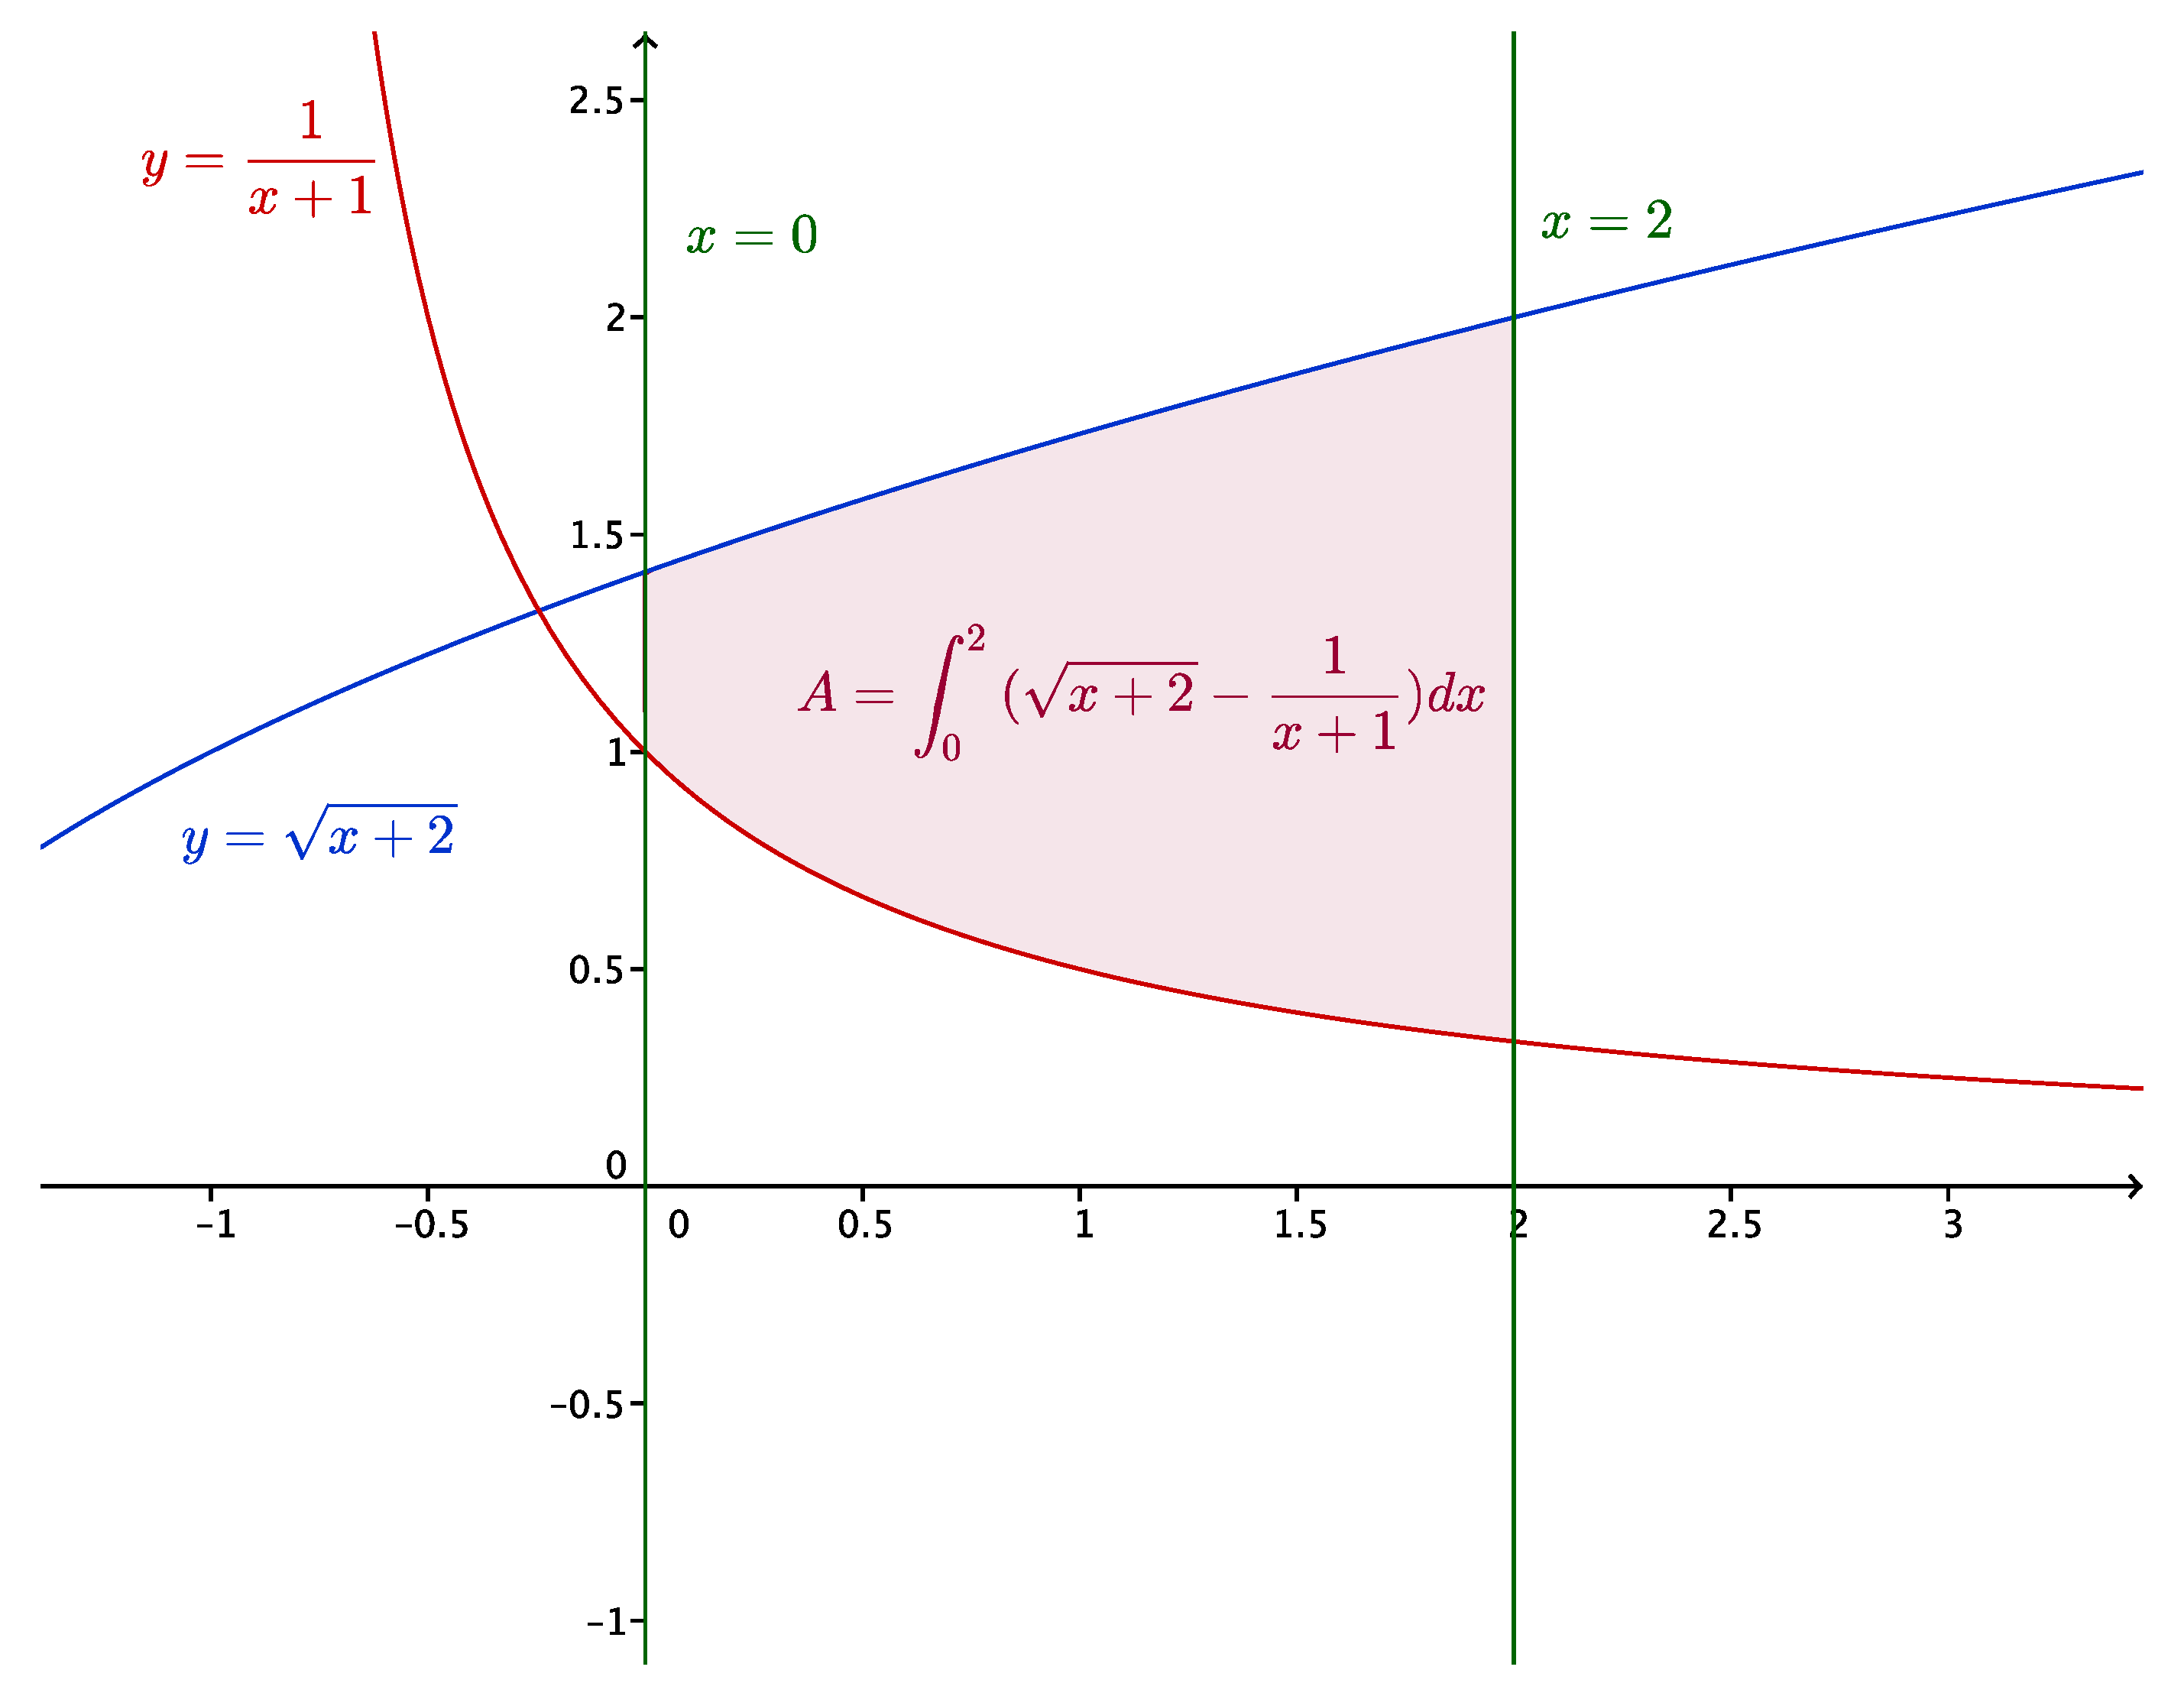
\includegraphics[width=0.8\textwidth]{WS4-1a}
 \end{center}
From the sketch we can see that $y=\sqrt{x+2}$ is the upper curve, and that there are no points of intersection between the given limits of integration. The area is therefore given by

\[
 A = \int_0^2\left((x+1)^{1/2}-\frac{1}{x+1}\right)\,dx = \left.\frac{2}{3}(x+2)^{3/2}-\ln(x+1)\right|_0^1 = \frac{16-4\sqrt{2}}{3}-\ln(3).
\]

 \item $y=2x^2+5x-3$ and $y=x^2+4x-1$.
 
  \begin{center}
  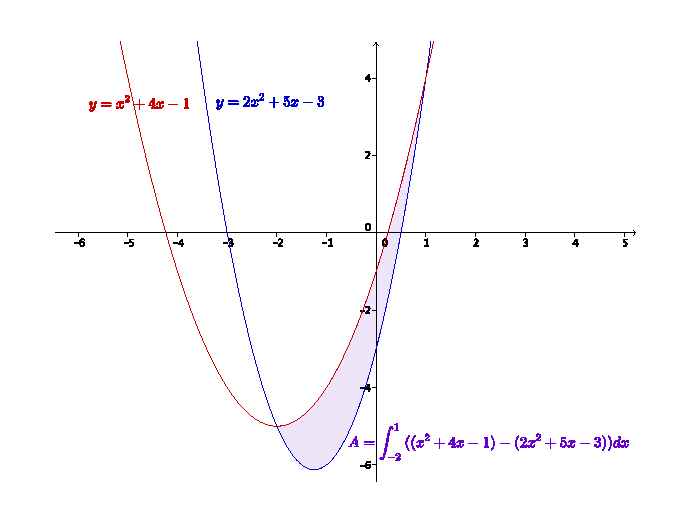
\includegraphics[width=0.8\textwidth]{WS4-1b}
 \end{center}
We see that the two curves intersect when $2x^2+5x-3=x^2+4x-1$, so $x^2+x-2=(x+2)(x-1)=0$, giving $x=-2, y=-5$ and $x=1, y=4$ as points of intersection. We also see that $(2x^2+5x-3)-(x^2+4x-1)=x^2+x-2<0$ for $-2<x<1$, giving us $y=x^2+4x-1$ as the upper curve. The area is therefore

\[
 A = \int_{-2}^1[(x^2+4x-1)-(2x^2+5x-2)]\,dx = \int_{-2}^1(2-x-x^2)\,dx = \left. 2x-\frac{x^2}{2}-\frac{x^3}{3}\right|_{-2}^1 = \frac{9}{2}.
\]

\pagebreak

  \item $y=x$ and $y=x^3$.
  
  \begin{center}
 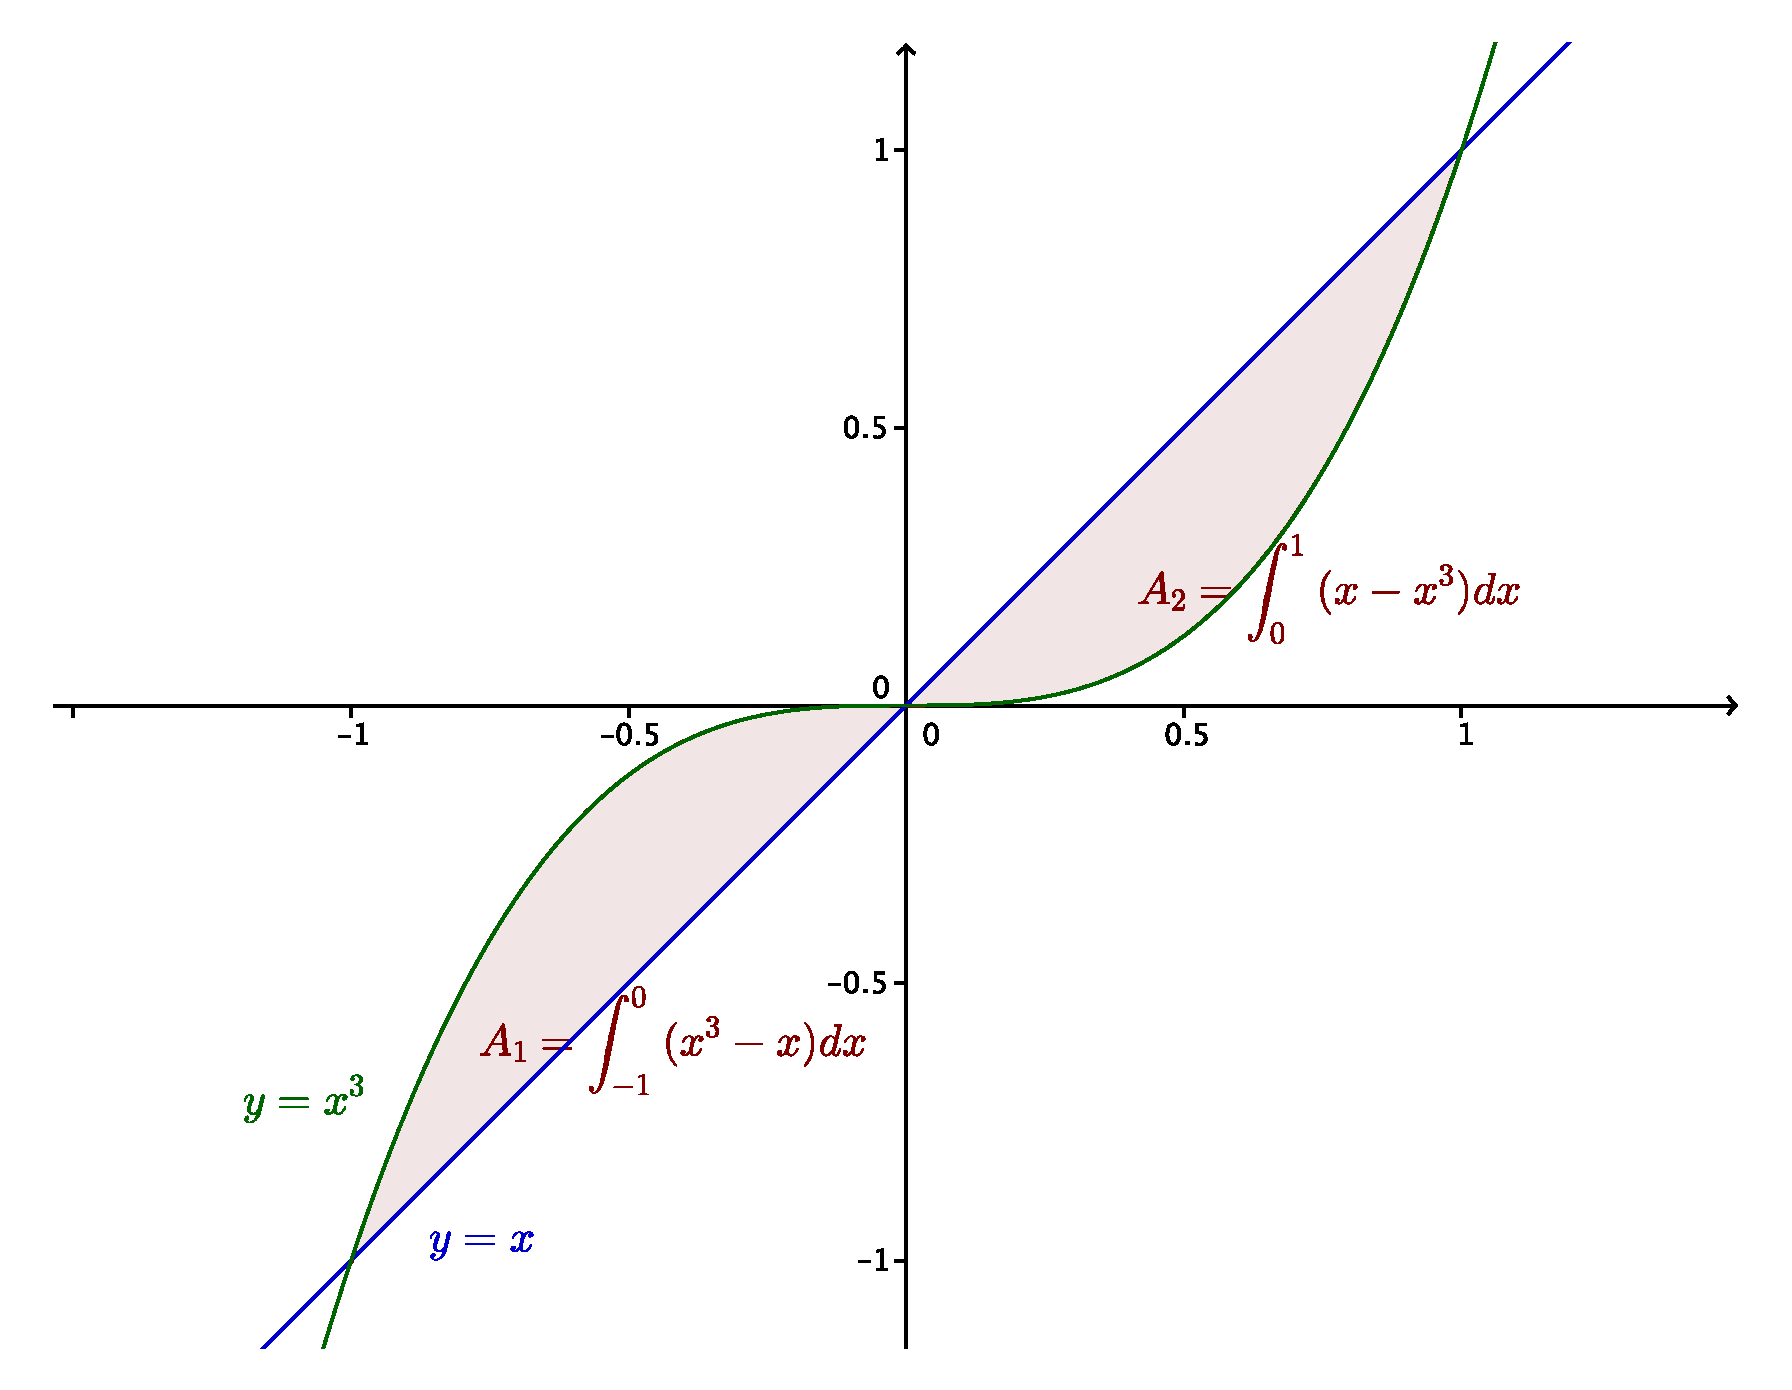
\includegraphics[width=0.8\textwidth]{WS4-1e}
\end{center}

The curves intersect if $x^3=x$, or $x^3-x = x(x-1)(x+1)=0$. There are thus two regions enclosed: the region below $y=x^3$ and above $y=x$, for $-1\leq x\leq 0$, and the region below $y=x$ and above $y=x^3$, for $0\leq x\leq 1$. By symmetry (both functions are odd), the areas of the two regions are equal. The area is therefore
\[
 A =2\int_0^1(x-x^3)\,dx = 2\left.\left(\frac{x^2}{2}-\frac{x^4}{4}\right)\right|_0^1 = \frac{1}{2}.
\]

\pagebreak

   \item $y=x^2+1$, $y=\frac{1}{4}(x-3)^2+1$, and $y=1$.
   
    \begin{center}
  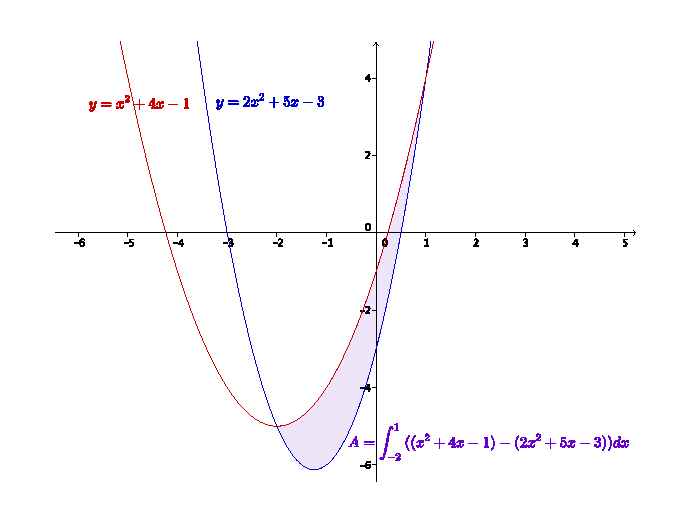
\includegraphics[width=0.8\textwidth]{WS4-1b}
 \end{center}
We see that the two curves intersect when $2x^2+5x-3=x^2+4x-1$, so $x^2+x-2=(x+2)(x-1)=0$, giving $x=-2, y=-5$ and $x=1, y=4$ as points of intersection. We also see that $(2x^2+5x-3)-(x^2+4x-1)=x^2+x-2<0$ for $-2<x<1$, giving us $y=x^2+4x-1$ as the upper curve. The area is therefore

\[
 A = \int_{-2}^1[(x^2+4x-1)-(2x^2+5x-2)]\,dx = \int_{-2}^1(2-x-x^2)\,dx = \left. 2x-\frac{x^2}{2}-\frac{x^3}{3}\right|_{-2}^1 = \frac{9}{2}.
\]
 \end{enumerate}

\end{enumerate}

\newpage
%\thispagestyle{empty}

\textbf{Assigned problems:}


 \begin{enumerate}

\item Evaluate the improper integral, if possible:

\begin{enumerate}
\item $\di \int_1^\infty\frac{\ln(x)}{x^2}\,dx$

Integrating by parts,
\[
\int \frac{\ln(x)}{x^2}\,dx = -\frac{\ln(x)}{x}+\int\frac{1}{x^2}\,dx = -\frac{\ln(x)}{x}-\frac1x,
\]
so 

\begin{align*}
\int_1^\infty\frac{\ln(x)}{x^2}\,dx& = \lim_{b\to \infty}\left(\left.-\frac{\ln(x)}{x}-\frac1x\right|_1^b\right)\\
& = \lim_{b\to \infty}\left(1-\frac{\ln(b)}{b}-\frac{1}{b}\right)=1,
\end{align*}
since $\lim_{b\to\infty}1/b=0$ and
\[
\lim_{b\to\infty}\frac{\ln(b)}{b} = \lim_{b\to\infty}\frac{1/b}{1}=0,
\]
using l'Hospital's rule.

\item $\di \int_0^\infty\frac{1}{e^x+e^{-x}}\,dx$

First, we note that
\[
\int \frac{1}{e^x+e^{-x}}\,dx = \int\frac{e^x}{e^{2x}+1}\,dx = \int\frac{1}{u^2+1}\,du = \arctan(e^x)+C,
\]
using the substitution $u=e^x$. Alternatively,
\[
\int\frac{1}{e^x+e^{-x}}\,dx = \frac12\int\sech(x)\,dx=\frac12\arctan(\sinh(x))+C,
\]
using a table of integrals for $\int\sech(x)\,dx$. (The two answers are, of course, equal up to a constant.) 

Since $e^x\to \infty$ as $x\to \infty$, we have
\[
\int_0^\infty\frac{1}{e^x+e^{-x}}\,dx = \lim_{b\to\infty}(\arctan(e^b)-\arctan(e^0))=\frac{\pi}{2}-\frac{\pi}{4}=\frac{\pi}{4}.
\]
\end{enumerate}
\pagebreak

\item Determine whether or not the following improper integrals converge or diverge. Use either direct comparison or limit comparison, as appropriate.

\begin{enumerate}
\item $\di \int_1^\infty \frac{1}{\sqrt{x^2+x}}\,dx$

For $x$ large, we note that $\dfrac{1}{\sqrt{x^2+x}}\approx \dfrac{1}{\sqrt{x^2}}=\dfrac{1}{x}$. Since $\di\int_1^\infty\frac{1}{x}\,dx$ diverges, we suspect that our original integral must diverge as well.

Unfortunately, since $x^2+x>x^2$ for $x>0$, $\frac{1}{\sqrt{x^2+x}}<\frac{1}{x}$, so direct comparison with $\dfrac{1}{x}$ is of no use. However, since $x^2>x$ for $x>1$, we have
\[
x^2+x<x^2+x^2=2x^2, \text{ so } \frac{1}{\sqrt{2x^2}}=\frac{1}{\sqrt{2}x}<\frac{1}{\sqrt{x^2+x}},
\]
and since $\di \int_1^\infty\frac{1}{\sqrt{2}x}\,dx = \frac{1}{\sqrt{2}}\int_1^\infty\frac{1}{x}\,dx$ diverges, our original integral must also diverge, by direct comparison.

If you weren't able to come up with a direct comparison, a limit comparison is also possible. With $f(x) = \dfrac{1}{\sqrt{x^2+x}}$ and $g(x) = \dfrac{1}{x}$, we have
\[
\lim_{x\to\infty}\frac{f(x)}{g(x)} = \lim_{x\to\infty}\frac{x}{\sqrt{x^2+x}} = \lim_{x\to\infty}\frac{1}{\sqrt{1+1/x}}=1.
\]
Since $0<1<\infty$ and $\int_1^\infty g(x)\,dx$ converges, $\int_1^\infty f(x)\,dx$ converges as well.

\item $\di \int_0^1\frac{1}{\sqrt{x^2-x}}\,dx$

This integral is nonsense. For $x\in (0,1)$, $x^2-x<0$, so the square root is undefined.

For a less nonsensical problem, you could try $di\int_0^1\frac{1}{\sqrt{x-x^2}}\,dx$. This is improper at both limits of integration, so we write
\[
\int_0^1\frac{1}{\sqrt{x-x^2}}\,dx = \int_0^{1/2}\frac{1}{\sqrt{x-x^2}}\,dx+\int_{1/2}^1\frac{1}{\sqrt{x-x^2}}\,dx.
\]
When $x$ is near 0, we note that $\dfrac{1}{\sqrt{x-x^2}}\approx\dfrac{1}{\sqrt{x}}$, since $x^2$ is much smaller than $x$ sufficiently close to zero, so we suspect convergence, since $\int_0^{1/2}x^{-1/2}\,dx$ converges.

To set up a comparison, note that for $0<x<1/2$, we have $x^2<x/2$, and thus $-x^2>-x/2$, so $x-x^2>x-x/2=x/2$, and therefore
\[
\frac{1}{\sqrt{x-x^2}}<\frac{1}{\sqrt{x/2}}=\frac{\sqrt{2}}{\sqrt{x}}.
\]
Since $\di \int_0^{1/2}\frac{\sqrt{2}}{\sqrt{x}}\,dx$ converges, so does $\di \int_0^{1/2}\frac{1}{\sqrt{x-x^2}}\,dx$.

For $\di\int_{1/2}^2\frac{1}{\sqrt{x-x^2}}\,dx$, consider the substitution $u=1-x$. Note that $du=-dx$, $x=1-u$, and thus
\[
x-x^2 = x(1-x)=(1-u)u=u-u^2,
\]
but when $x=1/2$, $u=1/2$, and when $x=1$, $u=0$. Therefore,
\[
\int_{1/2}^1\frac{1}{\sqrt{x-x^2}}\,dx = \int_{1/2}^0\frac{-1}{\sqrt{u-u^2}}\,du = \int_0^{1/2}\frac{1}{\sqrt{u-u^2}}\,du.
\]
But other than the use of the variable $u$ rather than $x$, this last integral is identical to the one that we just determined converges.

We conclude that both halves of the integral converge, and therefore,  $\di\int_0^1\frac{1}{\sqrt{x-x^2}}\,dx$ converges as well.
\end{enumerate}

\item (For in-class discussion): how do you show that $\di\int_0^\infty \frac{x^n}{e^{x}}\,dx$ exists for any positive integer $n$?

First, we note that $\di\lim_{x\to \infty}\frac{x^n}{e^x}=0$ for any positive integer $n$. Intuitively this is clear, since $e^x$ grows faster than any power of $x$. To see that it's true in general, notice that when $n=1$, l'Hospital's rule gives
\[
\lim_{x\to \infty}\frac{x}{e^x} = \lim_{x\to \infty}\frac{1}{e^x}=0.
\]
For any $n>1$, l'Hospital's rule again gives
\[
\lim_{x\to\infty}\frac{x^n}{e^x}=\lim_{x\to \infty}\frac{nx^{n-1}}{e^x},
\]
provided the latter limit exists. But aside from the constant, this last limit is of the same form, with the power reduced by 1. 

We can now use an argument called \textit{mathematical induction}: since the result holds for $n=1$, and the result for any larger $n$ can be reduced to the result for $n-1$, we get the result for all $n$ by chain reaction: it's true for $n=2$ since it's true for $n=1$. It's true for $n=3$ since it's true for $n=2$, and so on.

The same principle lets us deal with the integral itself. Integrating by parts,

\[
\int x^ne^{-x}\,dx = -x^ne^{-x}+n\int x^{n-1}e^{-x}\,dx,
\]
so
\[
\int_0^\infty x^ne^{-x}\,dx = \lim_{x\to\infty}(-x^ne^{-x}) + n\int_0^\infty x^{n-1}e^{-x}\,dx = n\int_0^\infty x^{n-1}e^{-x}\,dx.
\]
Since $\int_0^\infty xe^{-x}\,dx$ converges (see the solution to 2(b) in the additional practice problems), so do all the rest, by mathematical induction.


\item Let $p(x)$ be any polynomial function. Does $\di \int_0^\infty \frac{p(x)}{e^x}\,dx$ converge or diverge? Justify your answer.

We can write $\di p(x)=\sum_{n=0}^Na_nx^n$ for some constants $a_0,a_1,\ldots, a_N$, for a polynomial of degree $N$. (Allowing the usual abuse of notation that when $n=0$, $x^0=1$, even though $x^0$ is undefined at zero.)

It follows that
\[
\int_0^\infty \frac{p(x)}{e^x}\,dx = \int_0^\infty \sum_{n=0}^Na_nx^ne^{-x}\,dx = \sum_{n=0}^N\int_0^\infty\frac{x^n}{e^x}\,dx,
\]
so our integral can be written as a linear combination of integrals that, by problem \#3, all converge.

\item Find the area between the given curves:
\begin{enumerate}
\item $y=\cos x$ and $y=\sin 2x$, between $x=0$ and $x=\pi/2$.

\begin{center}
 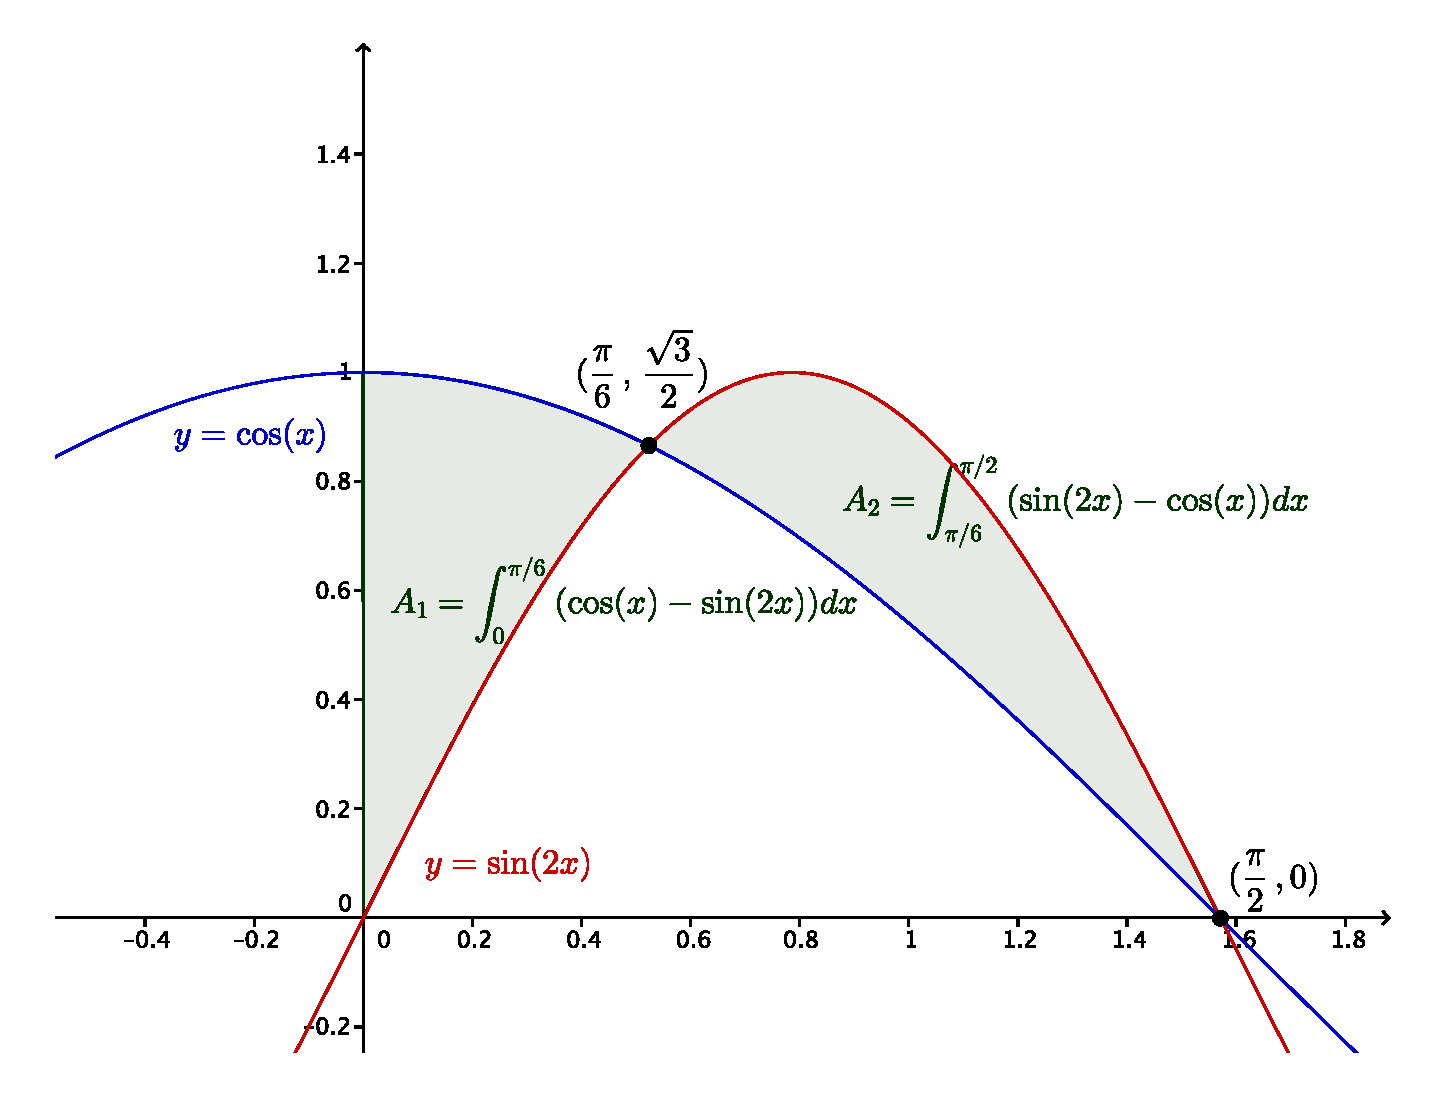
\includegraphics[width=0.8\textwidth]{WS4-1d}
\end{center}

From the sketch above, we see that the two curves change position once between $0$ and $\frac{\pi}{2}$, so we need to find the point of intersection. If $\cos x = \sin(2x) = 2\sin(x)\cos(x)$, we get $\cos(x)(2\sin(x)-1)=0$, so either $\cos(x)=0$ or $2\sin(x)=1$. On the interval $[0,\frac{\pi}{2}]$ we only have $\cos(x)=0$ when $x=\frac{\pi}{2}$, while $\sin(x)=\frac{1}{2}$ for $x=\frac{\pi}{6}$. The point of intersection is therefore at $x=\frac{\pi}{6}$, $y=\frac{\sqrt{3}}{2}$. The area is given by
\begin{align*}
 A & = \int_0^{\pi/6}(\cos (x) -\sin (2x))\,dx + \int_{\pi/6}^{\pi/2}(\sin(2x)-\cos(x))\,dx\\
& = \left.(\sin x+\frac{1}{2}\cos(2x))\right|_0^{\pi/6} + \left.(-\frac{1}{2}\cos(2x)-\sin(x))\right|_{\pi/6}^{\pi/2}\\
& = \frac{1}{2}+\frac{1}{4}-0-\frac{1}{2}-\frac{1}{2}(-1)-1+\frac{1}{4}+\frac{1}{2}\\
& = \frac{1}{2}.
\end{align*}

  \item $y=x$, $y=5x$, and $y=6-x^2$, in the first quadrant. 
  
  \begin{center}
 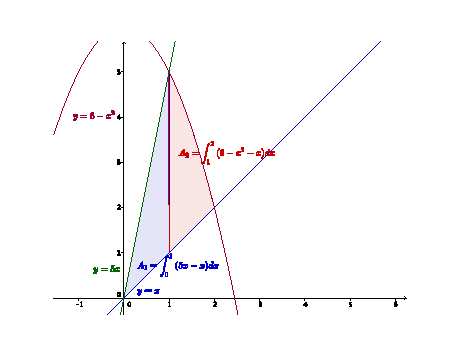
\includegraphics[width=0.8\textwidth]{WS4-1f}
\end{center}

Again we see that there are two areas to consider. The line $y=5x$ intersects the parabola $y=6-x^2$ when $6-x^2=5x$, or $x^2+5x-6 = (x+6)(x-1)=0$. The point of intersection in the first quadrant is therefore $x=1, y=5$. The line $y=x$ intersects the parabola $y=6-x^2$ when $6-x^2=x$, or $x^2+x-6=(x+3)(x-2)=0$. The point of intersection in the first quadrant is therefore $x=2, y=2$. The area is given by
\begin{align*}
 A & = \int_0^1(5x-x)\,dx + \int_1^2(6-x^2-x)\,dx\\
&=\left.2x^2\right|_0^1 + \left.\left(6x-\frac{x^3}{3}-\frac{x^2}{2}\right)\right|_1^2\\
&=\frac{25}{6}
\end{align*}
\end{enumerate}
\end{enumerate}
\end{document}